\section{Introduction}


Over the last decade, there has been a trend of individuals and organizations relocating their data from on-site storage such as workstations and file servers to off-site datacenters, colloquially known as ``cloud storage."  While there are economic benefits for doing so~\cite{CITATION NEEDED}, hosting data in an off-site datacenter introduces both latency and bandwidth performance penalties on reads and writes.  This is because with cloud-hosted data, read and write data must travel a longer physical distance, and pass through more networks (usually the public Internet) than it would otherwise have had to in order to reach on-site data stores.
\\
To overcome these performance penalties, both site operators and cloud operators employ network caches in order to make the data appear much closer to readers than it actually is.  Site operators employ caching proxies at their site's Internet connection, which fetch and cache data retrieved from an off-site source.  This way, on a cache hit, a read request is serviced from within the site's network, just as it would have been had the data been hosted on-site.  In addition, cloud operators employ \textit{content distribution networks} (CDNs) to cache data at regional \textit{Points of Presence} (PoPs) where the readers' ISPs peer with the ISPs that service the cloud.  Then, if there is a cache miss on the on-site cache, the reader's request may still be serviced by the PoP caches without being sent out of the ISP.  In both cases, the cloud appears to have been \textit{extended} to the reader's edge network:  despite the fact that the data is actually hosted in a datacenter, the read operation occurs as if the data was hosted within the ISP or the site itself.
\\
While it is well-known that network caches greatly improve read latency and bandwidth~\cite{Every CDN paper}, network cache implementations are not designed to improve write performance.  A write must always be sent to the cloud--the cloud is not extended to the edge of the network in the same way that it is for readers.  Additionally, most cache implementations require a reader to explicitly ask the cache to verify that the replica it will serve is fresh, and by default will serve potentially stale or even corrupted data in the presence of writers.  To remedy this, we propose Syndicate.
\\
Syndicate is a distributed storage service that extends cloud storage into edge networks.  A reader sends its request to its network-specific Syndicate \textit{Ingestion Gateway} (IG), which leverages existing proxies and CDNs to retrieve the data from its origin.  A writer sends data to its network-specific IG instead of the cloud, and Syndicate ensures that the data will eventually be replicated to the cloud.  However, as soon as data is committed to the IG, Syndicate ensures that any subsequent read on the data will return fresh bits, unless the reader explicitly allows for the possibility of stale data.

% Crisply state the advantages of Syndicate without reference to deployment scenarios or design (including the IG)
% User scenario: data center ex
\subsection{Motivation}

An organization would benefit from Syndicate if the read/write access patterns at each site had a degree of locality:  applications mostly read the same subset of data and write the same subset of data (although they need not intersect), but need to be able to read or write any record and have the changes be immediately visible.  Organizations additionally have a choice in where the IGs will be deployed:  as a process on the same host as each application, or as a site-wide service accessed via the local edge network.  To support the former, our IG implementation can be mounted as a FUSE filesystem (Figure~\ref{fig:syndicatefs-deployment}).  To support the latter, our IG implementation can also be run as an HTTP server (Figure~\ref{fig:syndicate-httpd-deployment}) to emulate the read/write Web API offerred by a cloud storage implementation.
\\
In either case, Syndicate is comprised of three components:

\begin{description}
\item[Ingestion Gateway:] The IG provides an interface to applications to read, write, host, and replicate data.
\item[Metadata server:] The metadata server is a cloud-hosted process which IGs use to discover each other's data and data replicas.
\item[Replica server:]  The replica server is a cloud-hosted process that receives data from IGs, puts the data into cloud storage, and serves the data to other IGs as needed.
\end{description}

A single deployment has a single metadata server, one or more IGs, and zero or more replica servers.

\begin{figure}[h!]
\centering
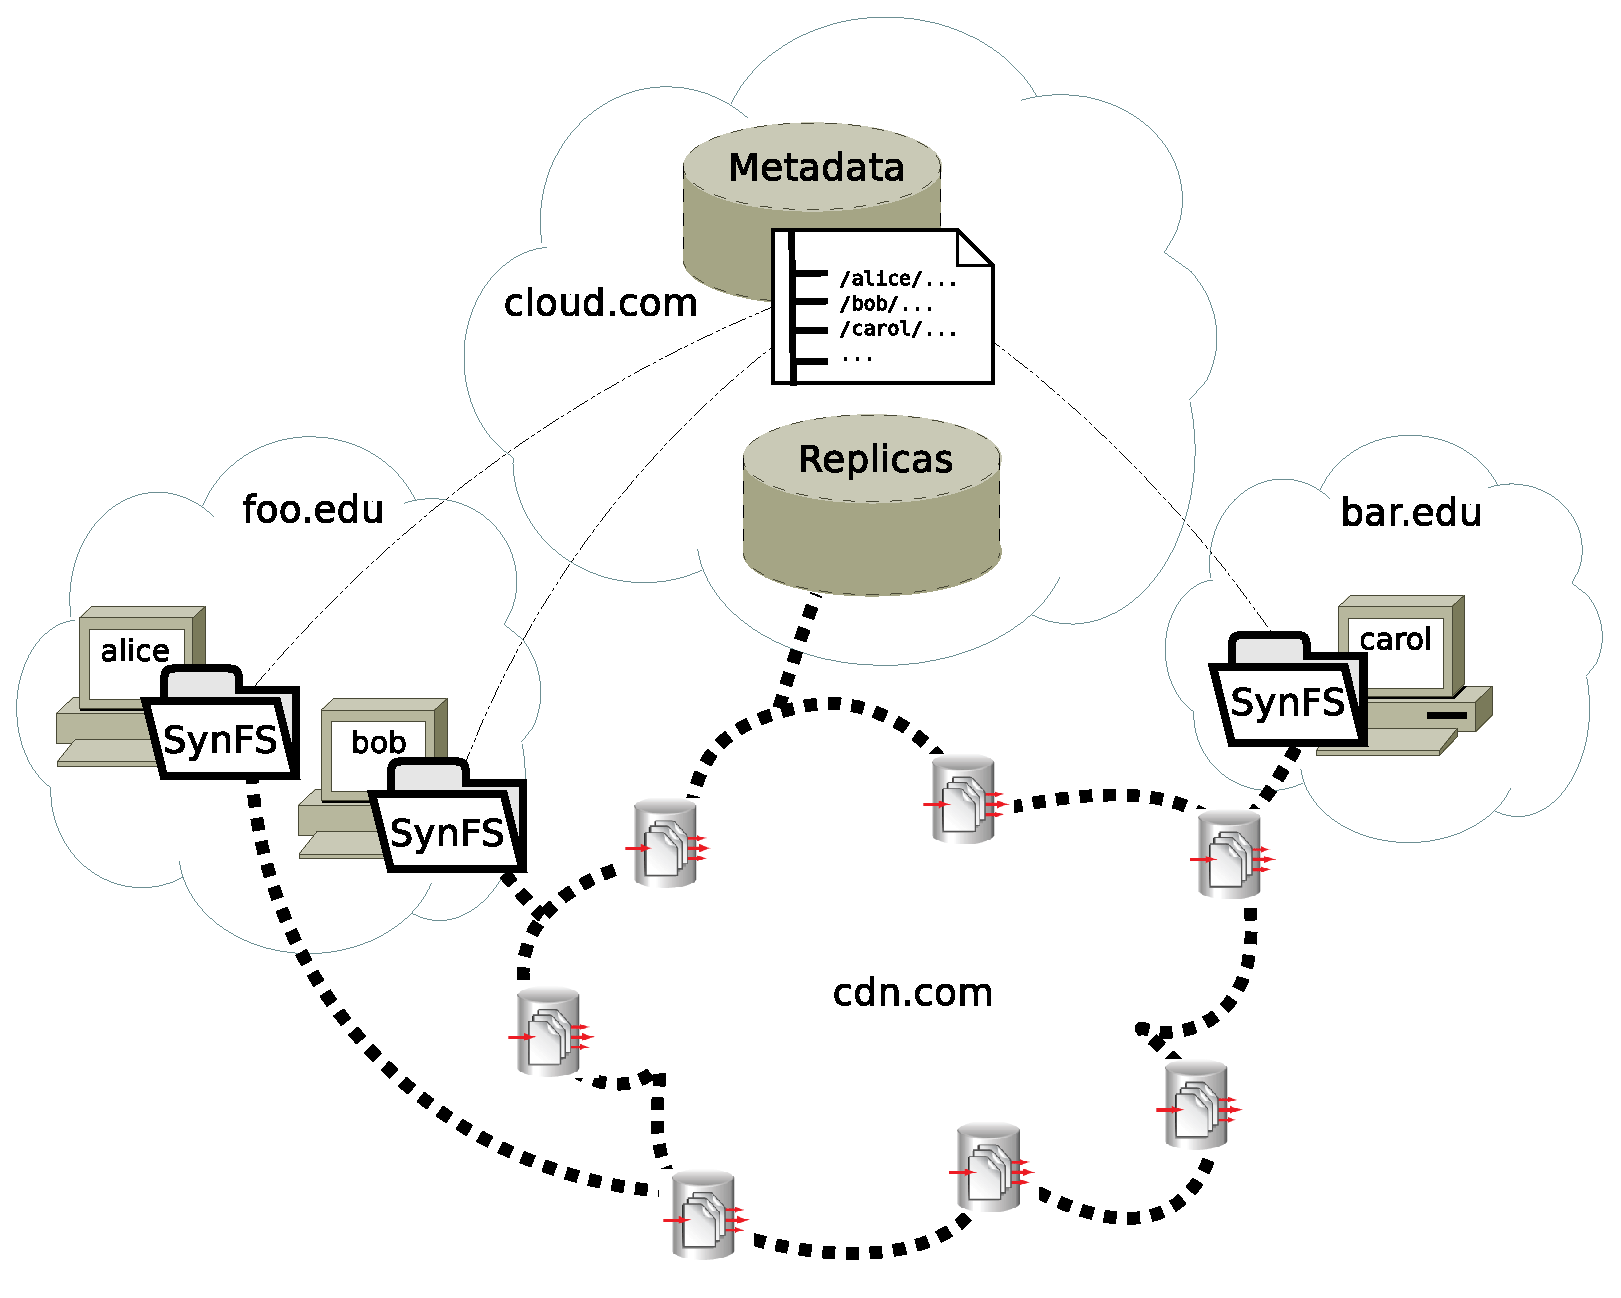
\includegraphics[width=0.5\textwidth]{figures/syndicatefs-deployment}
\caption{Structural overview of a Syndicate filesystem deployment with three clients, two at the same site and one at a remote site.  Each end-host sees every file between every host.  In this example, files created by the host \texttt{alice} are stored under \texttt{/alice/} (similar for \texttt{bob} and \texttt{carol}), but the scheme is arbitrary.}
\label{fig:syndicatefs-deployment}
\end{figure}

\begin{figure}[h!]
\centering
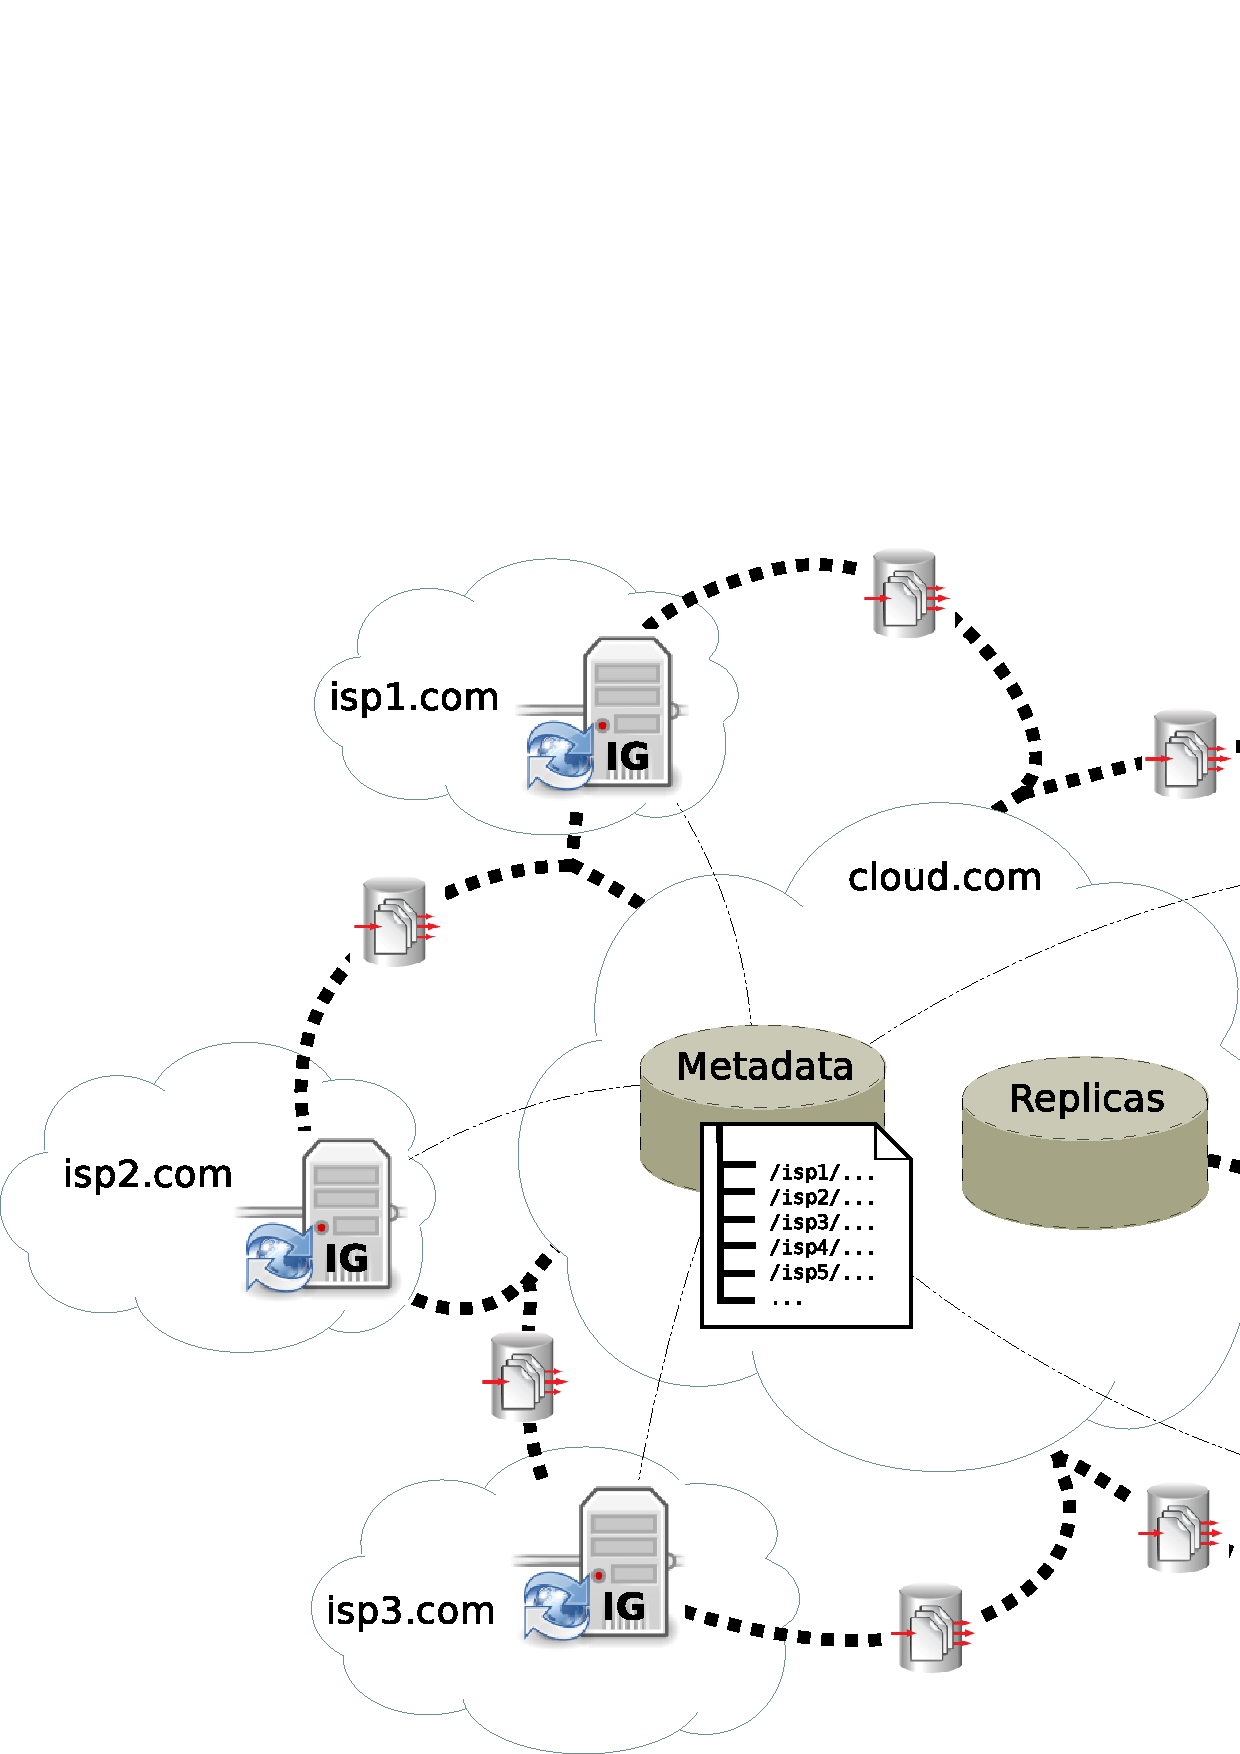
\includegraphics[width=0.5\textwidth]{figures/syndicate-httpd-deployment}
\caption{Structural overview of a Syndicate storage service deployment across five ISPs.  The server icons denoted "IG" denote the service's Ingestion Gateways, and the smaller file-marked storage icons denote CDN nodes.}
\label{fig:syndicate-httpd-deployment}
\end{figure}

\subsubsection{Syndicate as Local Storage}

When deployed as a filesystem, end-hosts use the IG to gain the ability to read and write data as a collection of files spread across cloud storage providers.  In implementation, locally-created data will be stored on the local host, and served to other IGs on demand.  This allows legacy applications to gain the benefits of Syndicate without needing to be re-written to use a cloud storage API, exposes data to users via the familiar file/folder metaphor, and provides a familiar, consistent naming scheme for data.

For example, suppose the geneticist Alice in Figure~\ref{fig:syndicatefs-deployment} works on analyzing GenBank~\cite{GenBank} data and wishes to share her gene sequences with collaborators Bob and Carol.  To do this, Alice directs the output of her sequencing tools to a collection of files on her workstation's mounted Syndicate filesystem.  Once the files are created, both Bob and Carol can proceed to read and write to them.  Syndicate ensures that Alice will read any changes once Bob and Carol write them.  Neither Alice nor the site operators from \texttt{foo.edu} need to worry about network traffic spikes if there are many collaborators, since the both the cloud's CDN and the sites' proxies cache frequently-read data.

As another example, suppose the workstations at \texttt{foo.edu} and \texttt{bar.edu} run hypervisors such as Collective~\cite{Collective}, which fetch and save a user's virtual machine image to and from a central NFS~\cite{NFS} server.  If the site operators were to replace the NFS client with a Syndicate client, and the NFS server with cloud storage, the unmodified hypervisors could greatly reduce their load and save times since they would fetch most of the VM's blocks from the CDN and site proxies.  Modified blocks and pages would be committed to the local IG and then uploaded asynchronously, reducing write latency.

Additionally, suppose that every night a cloud-based computer cluster (not shown) and a grid computing system (not shown) both ran batch jobs on the gene sequences generated the previous day.  In both cases, the compute nodes simply mount a Syndicate IG as a filesystem with the same metadata server as Alice, Bob, and Carol, and transparently read the data either from the researchers' workstations (if they are still turned on) or from the cloud-based replica server.  Only the relevant bits are streamed into the CDN and site proxies, and repeatedly-requested blocks of data are cached (i.e. multiple jobs touch the same data).

\subsubsection{Syndicate as Web Storage}

When deployed as a site-wide Web-accessible storage service, Syndicate acts as a read/write front-end for site's cloud storage provider.  For example, suppose that \texttt{isp1.com} in Figure~\ref{fig:syndicate-httpd-deployment} is a city-wide cellular network, and the IG is deployed at the PoP where the cellular network is connected to the Internet.  Then, most location-aware smartphone applications, such as those for maps, picture and video sharing, messaging, geocaching, social collaboration, and augmented reality, which today use cloud storage providers to store and distribute their data, can instead use a much-closer IG for the same purpose.  In these cases, smartphone users in the same geographic region (and thus the same cellular network) tend to mostly read and write data relating to their region (e.g. their friends' data, local venue data, etc.).  With Syndicate, smartphone application developers would partition their data by geographic regions to ensure that groups of smartphone users in the same network read and write to the same IG.


Syndicate might also be used as a platform for accelerating web applications.  Today, web applications usually read and write records in a nearby (even local) database server on behalf of remote users.  If a web application can tolerate sequential consistency of reads and writes on its records, and if an application server usually reads and writes from the same rows and tables, a web deveoper could deploy the web application on servers within PoPs instead of the cloud, and use a Syndicate IG in the PoP to mediate reads and writes to a cloud-hosted DBMS.  Since the application servers in the PoP read and write the same records frequently, most read and write requests can be processed by the IG in the PoP on behalf of the cloud, yielding much faster read and write performance.  One class of beneficiaries would be distributed social network platforms such as Diaspora~\cite{Diaspora}, which usually read and write rows and tables relating to a user's personal data and friends' personal data.  Another class of beneficiaries is edge network management software for wide-are federated systems such as ProtoGENI~\cite{ProtoGENI} and PlanetLab~\cite{PlanetLab}--a Syndicate IG in the edge network's PoP could serve as a front-end for the globally central database that represents the set of edge networks' states.  Edge nodes would read and write their state information to IG instead of the central database, and Syndicate would ensure that all other IGs, as well as the central database, would see only fresh state information from the edge nodes.

There are more examples of how Syndicate might be used, but we omit them here for brevity.  The remainder of this paper is organized as follows:



